\section*{Introduction}
\phantomsection\label{sec:Introduction}
\addcontentsline{toc}{section}{Introduction}
\glsresetall

This article investigate a super model \citep{struttTheorySound1877}. 
You can use acronyms defined in acronyms.tex, for example \acp{MSA}.
Text continue ...
Another acronym (defined in acronym.tex) \ac{AM}.

An example figure 

\begin{figure*}
	\centering
	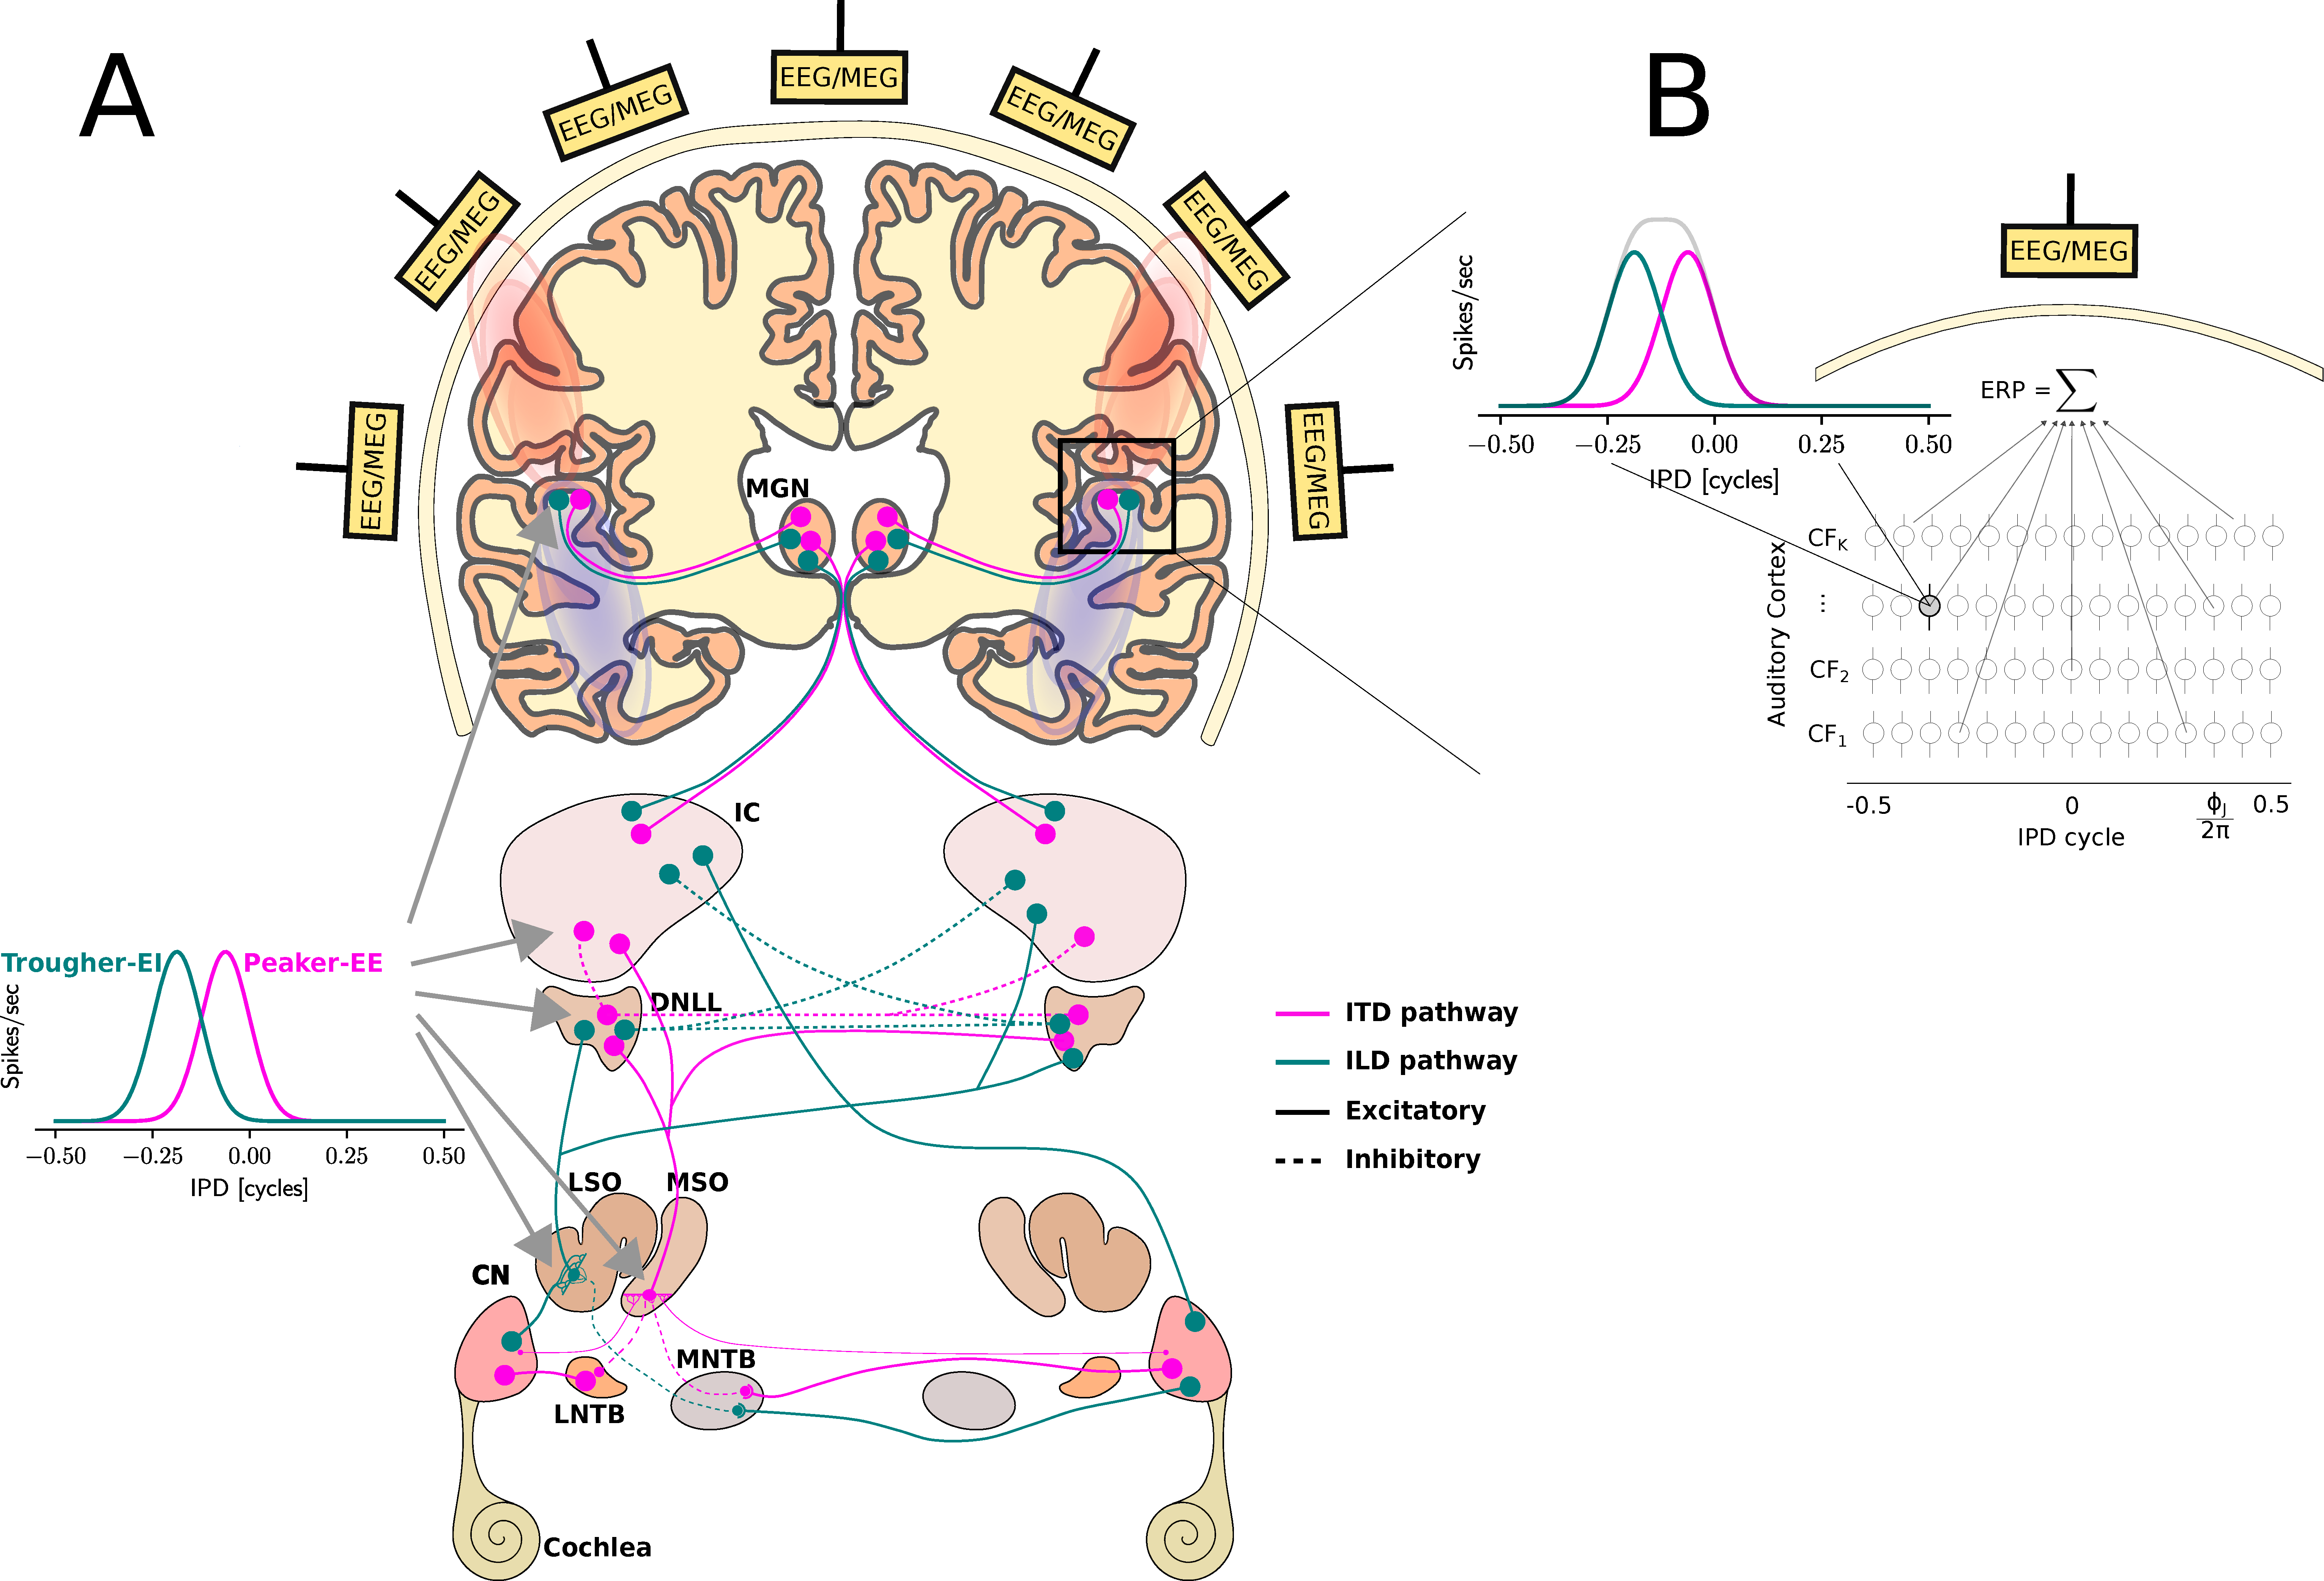
\includegraphics[width=16cm]{./figures/figure_example.pdf} % your figure should be in figure folder
	\caption{
	\textbf{\color{Black}Figure experiment heading.}
	\textbf{A}, this figure shows a model from Undurraga et al. 2023
	\textbf{B}, another panel
	}
	\label{fig:example_figure_0}
\end{figure*}

\lipsum[1-4]